\documentclass[12pt]{extarticle}
\usepackage{tikz}
\usepackage{amsmath,amssymb}
\usepackage {graphicx}
\usepackage{multicol}
\usepackage{hyperref}
\usepackage{geometry}
\usepackage{watermark}
\usepackage{varwidth}
\usepackage{arydshln}
\usepackage[dvipsnames]{xcolor}
\usepackage{tcolorbox}
%\usepackage{scrlayer-scrpage}
\usepackage{forest}
\usepackage{fancyhdr}
\pagecolor{white}
 \geometry{bottom= 30mm}
\usepackage{enumitem}


 
 
\title{Data Management Assignment 5}
\author{Cuihuan Zhang \& Janis Waser} 
\fancyhead[L]{Data Management}
\fancyhead[C]{Homework 5}
\fancyhead[R]{Cuihuan Zhang \& Janis Waser}
\renewcommand\headrulewidth{0pt}
\pagestyle{fancy}
\pagenumbering{arabic}

\begin{document}

\maketitle \vspace{-10mm}
\rule{\linewidth}{0.4pt}


\begin{flushleft}
\begin{enumerate}[label=\textbf{\Alph*.}]

\item 
\begin{enumerate}[label=\arabic*)]
\item \begin{enumerate}[label=(\alph*)]
\item If we are inserting at the beginning of a heap it takes only 1 operation. 
\item If we have no pointer to the back, it takes N operations to get there and insert the value.
\end{enumerate}
\item It takes log N operations to find the position where the value has to be inserted if the sequence is balanced (no overflow values). Unless the inserted value belonged to the end for example if a new maximum was inserted in which case the moving would not be necessary, every value which position is after in the sequence (tail) has to be moved taking N operations.  Added up this gives us log N + N operations. 
\item In a 2-3 tree it always takes O(log N) operations to insert a value. Either the inserted value can be positioned at the lowest level for which one has to go down the tree to find the place, and since the tree is guaranteed to be balanced it takes exactly log N steps.

The other case is where there is no place at the lowest level and therefore value have to propagate up, but again it takes log N operations in the worst case to go up the entire tree this gives us log N + log N steps which in the big-O notation is also O(log N).
\end{enumerate}
\item \begin{enumerate}[label=\arabic*)] 
\item If for every key there exists a pointer to the file where the key is stored, we call it a dense index, sparse otherwise. So it is a dense index if every key is indexed. 
In our example we see a dense index if we ignore the six, but if any key would miss in the index and therefore also its arrow were not present it would be sparse. If we were to include the six as part of a file then it would be sparse because not every key is in the index.
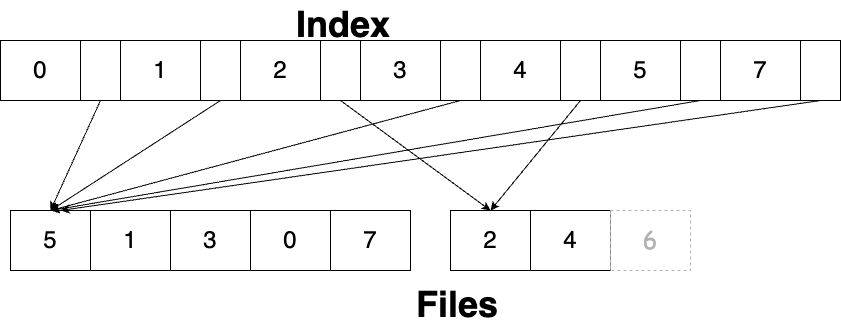
\includegraphics[width=\linewidth]{dense}
\item If every key that is in between two indexed keys is stored in the same file then we call it a clustered file, if this is not the case then it is unclustered. In our example we see a clustered example. Note that the files are not necessarily ordered within but they all lie in a range(they are grouped/"clustered"). In every other file all the keys are either strictly bigger or smaller. 
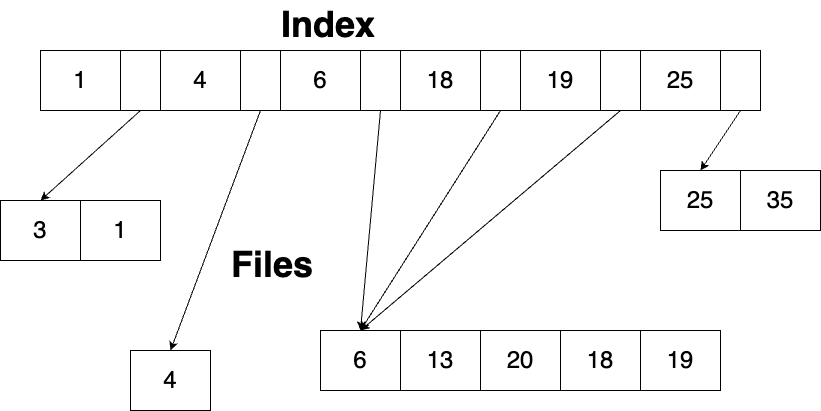
\includegraphics[width=\linewidth]{clustered}
The example in B 1 was obviously unclustered, as 3 is in another file than the file with 2 and 4, which in turn also violates the existence of the file with 0,1 and 5,7 in the same file. If we correct this we receive a dense clustered index:
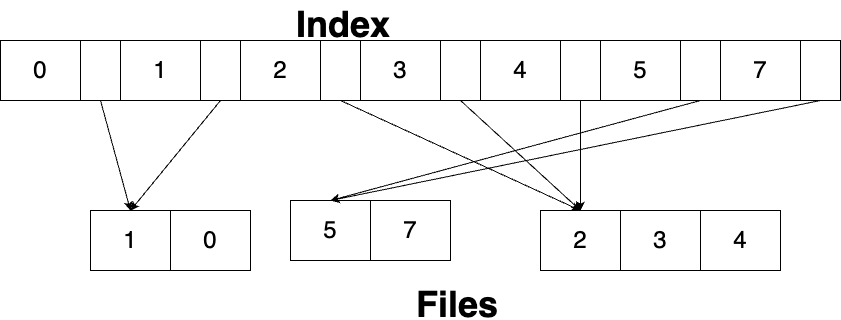
\includegraphics[width=\linewidth]{densecluster}
\item Sparse index and unclustered file is the worst choice, since to find any record you potentially have to search all files because you cannot always know in which file the key is stored.

A dense index and clustered file works but also has some flaws. The main concern is that the index is unnecessarily big when it would be enough to omit some. 

Now, we can either have dense index and unclustered file or sparse index and clustered file. For the first option, with dense index we can easily find the record but maybe the index is still unnecessarily big but  at least we did not to bother clustering the files which might require some resources.

 The best solution is a sparse index and clustered file. It is still easy to find the key as you search the pointer which contains the range of it and you do not store all keys in the index. Not all the keys are in the index and therefore less storage and maintenance is required.
\end{enumerate}
\item \begin{enumerate}[label=\arabic*)] 
\item We have 5 GiB on the disk this is $5\times 2^{30}$ bytes. Each block holds $256 = 2^8$Bytes. Therefore we have $\frac{5\times 2^{30}}{2^8}= 5\times 2^{22}= 1.25\times 2^{24}\leq 2^{25}$ blocks. We round up to make easier calculation and ensure that all addresses can be covered. We allocate 4 bytes to the block address(pointer size), which is little bit more than actually needed. 

Each node in the B-tree contains an amount m of pointers and (m-1) keys. The key size is 8 bytes from the ID. Therefore, the largest possible value for m can be calculated:

$ m \times (pointer size) + (m-1) \times (key size)\leq block size$

$m \times 4+ (m-1) \times 8 \leq 256 \Leftrightarrow 12m\leq264\Leftrightarrow m\leq 22$

We see the largest possible value of children is 22(no rounding necessary). This means the minimum number of children for internal nodes is 11. 
\item 
We have 5'000'000 records. 

\begin{tabular}{lll}
\hline
Level & Nodes in a narrow tree (\(m=11\))& Nodes in a wide tree (\(m=22\))\\
\hline
1     & 1          & 1          \\
2     & 2          & 22         \\
3     & 22         & 484        \\
4     & 242        & 10'648     \\
5     & 2'662      & 234'256    \\
6     & 29'282     & 5'153'632\\
7     & 322'102    & 113'379'904\\
8     & 3'543'122  & 2'494'357'888\\
9	& 38'974'342&54'875'873'536\\
\hline
\end{tabular}

In the narrowest tree 8 levels with $3'543'122\times 11=38'974'342$ pointers are more then enough, 7 levels are actually enough as some nodes will have more then 11 nodes even though $ 322'102\times 11 = 3'543'122$ is less than the required 5 million. Some nodes have more leaves to compensate.

In the widest tree 5 levels with $234'256 \times 22=5'153'632$ is a little bit too much but is also fine, since we have some fewer leaves coming out which is not violating the tree such that we have precisely 5 million pointers.  

Therefore, the tree has a range of 5 to 7 levels.
\item We are interested in range search. Hashing is a bad idea because with a good hash you would have to search all potential values in the range and if this is a continuous range, you would need search through every single file, if were to create secondary index for name this would be a good idea. In a $B^+$-tree on the other hand you could cluster easily on quantity and you have to access only a few blocks corresponding to the searched range. 

\end{enumerate}

\item We read R once and compare with S which needs to be done 1000 times (2000/2), this gives: read R + read 500/4 S$= 2000 + 1000\times4000=4'002'000$.

We read S once and compare with R(4000/4 times ): $4000+ 1000 \times 2000=2'004'000$, since this option requires less operations we prefer this one.
%The other option is where you read S first and compare 1000 (4000/4) times with R  this gives read S+ read 1000 R= 4000/4+ 1000*2000/2=1'001'000. The second option is considerably worse hence we opt to read R and compare with S.
\end{enumerate}
\end{flushleft}
\end {document}